\section{Backpropagation}

\subsection{Notation}

Um in einem mehrschichtigen Netz effizient die Kostenfunktion zu minimieren wird in vielen Fällen der \emph{Backpropagation}-Algorithmus verwendet. Dieser wurde bereits in den Siebzigerjahren definiert, erlangt jedoch erst im Jahr 1986 mit dem Paper \emph{Learning representations by back-propagating errors} von Rumelhart, Hinton und Williams Bekanntheit. 

Im vorherigen Teil habe ich bereits beschrieben was man unter dem Gradientenabstieg versteht und wie dieser auch bei mehrdimensionalen Funktionen (wie zum Beispiel der hierbei betrachteten Kostenfunktion) verwendet werden kann. Es wurde jedoch noch nicht vorgestellt, wie man auf ein mehrschichtiges Netz bezogen, diesen Gradienten überhaupt berechnen kann. 

Gemeinhin wird die Notation wie sie in Abbilung \ref{fig:weight_not} zu sehen ist, für ein Gewicht verwendet. In Abbildung \ref{fig:biasAct_not} steht das $b^l_j$ für den Schwellwert (\emph{Bias}) am Neuron mit dem Index \emph{j} im Layer mit dem Index \emph{l}. Selbes gilt für die Aktivierung welche mit einem \emph{a} gekennzeichnet wird. Mit den gegebenen Notationen können wir folgende Gleichung für die Aktivierung eines Neurons aufstellen (siehe Gleichung \ref{eq:act}). 

\begin{figure}[!htb]
	\centering
	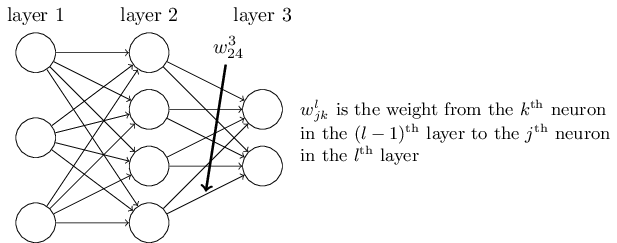
\includegraphics[width=.9\linewidth]{img/weight_notation}
	\mycaption{Notation}{dlnielsen}
	\label{fig:weight_not}
\end{figure}

\begin{figure}[!htb]
	\centering
	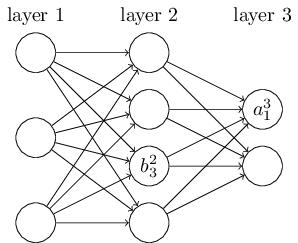
\includegraphics[width=.4\linewidth]{img/biasAct_notation}
	\mycaption{Notation}{dlnielsen}
	\label{fig:biasAct_not}
\end{figure}

\begin{equation} \label{eq:act}
a^{l}_j = \sigma\left( \sum_k w^{l}_{jk} a^{l-1}_k + b^l_j \right),
\end{equation}

Diese Formel sollte bereits aus den vorherigen Kapiteln bekannt sein. Es wird hierbei lediglich eine Vektormultiplikation der beiden eingehenden Gewichtsvektors und Addition mit den Aktivierungsvektoren durchgeführt. Die generierte Ausgabe wird mit dem Schwellwert verrechnet und in eine Aktivierungsfunktion (wie sum Beispiel der Sigmoid-Funktion) gesteckt.

Um später einfacher mit all diesen Werten zu rechnen wird versucht die gegebenen Werte in eine Matrix- beziehungsweise Vektor-Darstellungsform zu bringen. Da Neuron mehrere ausgehende \myquote{Pfade} besitzen wird hierbei eine Matrix geformt. Das bisher beschriebene Gewicht $w^l_{jk}$ befindet sich hierbei in der Zeile mit dem Index \emph{j} und Spaltenindex \emph{k}. Da sich sowohl der Schwellwert als auch die Aktivierung lediglich auf ein einzelnes Neuron beziehen muss hierfür lediglich ein eindimensionaler Vektor pro Layer \emph{l} generiert werden. Die einzelnen Komponenten werden hierbei über den Index \emph{j} angesteuert. Die Notation für den Aktivierungsvektor der Schicht \emph{l} sieht dann derartig aus: $a^l_j$. Ähnliches gilt fur die Schwellwerte: $b^l_j$. 

Um mit diesen Vektoren arbeiten zu können muss man die abschließende Aktivierungsfunktion $\sigma$ vektorisieren 
\footnote{Klarer Verweis auf Nielsen Buch, Kapitel über Backpropagation im Detail \cite{dlnielsen}}. 
Dabei muss man die Funktion lediglich derartig umschreiben, dass diese auf die einzelnen Komponenten angewendet wird und nicht auf einen einzelnen Wert. Beispielsweise würde die Funktion $f(x) = x^2$ vektorisiert folgendermaßen aussehen: 

\begin{equation}
  f\left(\left[ \begin{array}{c} 2 \\ 3 \end{array} \right] \right)
  = \left[ \begin{array}{c} f(2) \\ f(3) \end{array} \right]
  = \left[ \begin{array}{c} 4 \\ 9 \end{array} \right],
\end{equation}

Mit diesen Zusammenfassungen kann nun die Gleichung \ref{eq:act} folgendermaßen umgeschrieben werden: 

\begin{equation}
  a^{l} = \sigma(w^l a^{l-1}+b^l).
\end{equation}

Diese Umschreibung abstrahiert das Denken über die lokalen Neuronen auf ein höheres Level sodass es einfacher ist das Gesamtbild zu betrachten. Um noch mehr Klarheit zu schaffen wird oftmals die Aktivierung einer Schicht \emph{l} aus der Funktion herausgezogen und mit dem Buchstaben \emph{z} versehen. $z^l$ kann nun in die Aktivierungsfunktion $\sigma$ eingesetzt werden. Im folgenden habe ich noch einmal alle bisherigen Erkenntnisse zusammengefasst: 

\begin{mytheo}{Backpropagation - Notation}{theoexample}

Bisherige Schreibweise:
\begin{equation}
  a^{l}_j = \sigma\left( \sum_k w^{l}_{jk} a^{l-1}_k + b^l_j \right) \nonumber
\end{equation}

Zusammengefasste Form:
\begin{equation}
a^l = \sigma(z^l)
\end{equation}

Gewichtete Eingabe:
\begin{equation}
  z^l \equiv w^l a^{l-1}+b^l
\end{equation}

\end{mytheo}

\subsection{Fundamentale Gleichungen}

Ziel des Backpropagation Algorithmus ist es herauszubekommen welche Gewichte und Schwellwerte verändert werden müssen um die Kostenfunktion zu minimieren. Im folgenden werde ich nach und nach die vier wichtigsten Formeln des Verfahrens beschreiben. 

\begin{mytheo}{Backpropagation - Fundamentale Gleichungen}{theoexample} \label{theo:zus}

\begin{equation} \label{eq:error}
\delta^L = \nabla_a C \odot \sigma'(z^L).
\end{equation}

\begin{equation}
\delta^l = ((w^{l+1})^T \delta^{l+1}) \odot \sigma'(z^l),
\end{equation}

\begin{equation}
\frac{\partial C}{\partial b^l_j} = \delta^l_j.
\end{equation}

\begin{equation}
\frac{\partial C}{\partial w^l_{jk}} = a^{l-1}_k \delta^l_j.
\end{equation}

\end{mytheo}


\subsection{Fehler auf der Ausgabeschicht (Gleichung \ref{eq:error})}
Um zu verstehen was man unter einem Fehler genau versteht sei angenommen die Ausgabe eines Neurons \emph{j} im Layer \emph{l} wird um einen unbestimmten Wert verzerrt. Mathematisch ausgedrückt sieht dies dann folgendermaßen aus: 

\begin{equation}
\sigma(z^l_j+\Delta z^l_j)
\end{equation}

Statt der herkömmlichen Ausgabe $\sigma{z^l_j}$ wird ein \emph{Fehler} $\Delta z^l_j$ hinzugefügt. Allgemein wird der Fehler eines einzelnen Neurons dadurch folgendermaßen beschrieben: 

\begin{equation}
\delta^l_j \equiv \frac{\partial C}{\partial z^l_j}.
\end{equation}

Wie wir bereits beim Gradientenabstieg gesehen haben, beschreibt diese partielle Ableitung die \glqq Steigung \grqq der Kostenfunktion im Bezug auf den die Ausgabe $z^l_j$. Dieser Wert dient im späteren Verlauf allerdings lediglich als Zwischenschritt, da wir im Endeffekt an den Gradienten bezüglich der Gewichte sowie den Schwellwerten interessiert sind. Im Nachhinein wird daher versucht den Fehler ${\partial C / \partial z^l_j}$ auf die Gewichte ${\partial C / \partial w^l_j}$ und Bias ${\partial C / \partial b^l_j}$ zurückzuführen. 

Die komponentenweise Darstellung für die Berechnung des Fehlers auf der Ausgabeschicht $\delta^L$ sieht folgendermaßen aus:

\begin{equation}
\delta^L_j = \frac{\partial C}{\partial a^L_j} \sigma'(z^L_j)
\end{equation}

Der vordere Teil $\partial C / \partial a^L_j$ beschreibt wie sich die Kostenfunktion bezüglich eines Neurons mit dem Index \emph{j} auf der Ausgabeschicht verhält (Steigung der Kostenfunktion nach $a^L_j$). Wenn das Neuron nicht sehr viel \emph{Einfluss} auf die Kostenfunktion nimmt, bleibt dieser Faktor klein und das Ergebnisfehler fällt minimal aus. Der hintere Teil beschreibt die Ableitung der Aktivierungsfunktion und die Steigung an der gegebenen Stelle $z^L_j$. 
Da man hierbei auch wieder versuchen möchte die Formeln möglichst allgemein zu halten wird der Fehler auf wieder als Vektor der Ausgabeschicht definiert. Das sieht dann so aus: 

\begin{equation}
\delta^L = \nabla_a C \odot \sigma'(z^L)
\end{equation}

Dies ist auch die Darstellung wie sie Anfang des Abschnitts verwendet wurde (siehe \ref{theo:zus}). $\nabla_a C$ stellt dabei den Vektor dar dessen partielle Ableitung $\partial C / \partial a^L_j$ entsprechen. Es ist also lediglich eine andere Schreibweise für die partielle Ableitung bezogen auf die komplette Ausgabeschicht. Wenn wir für die Kostenfunktion wie schon in früheren Kapiteln die quadratische Kostenfunktion wählen entspricht \emph{C} gleich $C = \frac{1}{2} \sum_j (y_j-a^L_j)^2$. Nach $a^L_j$ abgeleitet entspricht dies dann wiederum $\partial C / \partial a^L_j = (a_j^L-y_j)$. Die Herleitung ist sehr ähnlich zu der des Gradienten (siehe \ref{deri:grad}), hier fehlt lediglich die Iteration über die kompletten Trainingsdatensätze. 

Der entstandene Vektor ($\nabla_a C$) wird dann komponentenweise mit der Ableitung der Aktivierungsfunktion multipliziert. Da diese vektorisiert wurde entspricht das Ergebnis von $\sigma'(z^L)$ ebenfalls wieder einem Vektor was diese Rechenoperation ermöglicht. Eine andere Schreibweise ist daher folgende Gleichung: 

\begin{equation}
\delta^L = (a^L-y) \odot \sigma'(z^L)
\end{equation}

Hierbei wurde lediglich die Ableitung eingesetzt. 